\documentclass{article}
\usepackage[T1]{fontenc}
\usepackage{lmodern}
\usepackage{graphicx}
\usepackage{amsmath,amssymb}
\usepackage[a4paper,margin=2cm]{geometry}
\usepackage[absolute,overlay]{textpos}
\setlength{\TPHorizModule}{1mm}
\setlength{\TPVertModule}{1mm}
\usepackage[indonesian]{babel}
\usepackage{hyperref}
\setlength{\emergencystretch}{2em}
% unit: Halaman 25

\begin{document}

% === Halaman 25 (llm) ===

\begin{itemize}
  \item Buatlah grafik dengan Microsoft Excell dengan menggunakan nilai-nilai desimal di atas
  \item Misalnya nilai-nilai tersebut menyatakan jumlah penderita demam berdarah selama 20 bulan di Kota Bogor (Januari 2017 -- Agustus 2018).
\end{itemize}

\vspace{10mm}

% deskripsi: Grafik batang yang menunjukkan jumlah penderita Demam Berdarah di Kota Bogor dari Januari 2017 sampai Agustus 2018.
% bbox normalisasi: [0.2010, 0.3450, 0.7860, 0.9840]
\begin{textblock*}{122.85mm}(42.21mm,102.46mm)
\noindent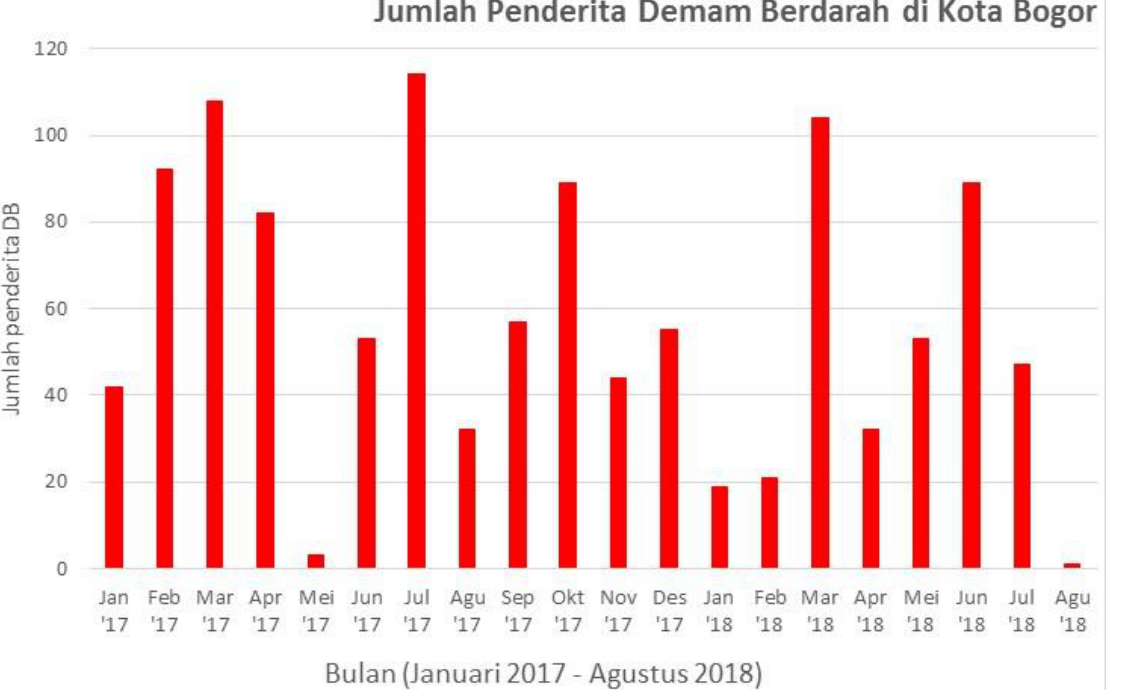
\includegraphics[width=122.85mm,height=189.78mm]{../../images/llm/page_025_img_01.png}%
\end{textblock*}

\end{document}
